\documentclass{article}
\usepackage{amsmath}  % 数学符号包
\usepackage{amssymb}  % 更多数学符号
\usepackage{enumitem} % 列表样式
\usepackage{fancyhdr} % 页眉设置
\usepackage{geometry} % 页面设置
% \usepackage[UTF8]{ctex}
\usepackage{bm}
\usepackage{amsthm}
\usepackage{graphicx}
\everymath{\displaystyle}  % 让所有数学模式都使用 \displaystyle
\newcommand{\lb}{\left\llbracket}
\newcommand{\rb}{\right\rrbracket}


\geometry{a4paper, margin=1in}


\pagestyle{fancy}
\fancyhf{}
\fancyhead[C]{Discrete Math Homework 17}
\fancyhead[R]{2024.12.22}


\title{Discrete Math Homework 17}
\author{noflowerzzk}
\date{2024.12.22}


\begin{document}
\maketitle

\section{}

\begin{enumerate}
    \item Choose a as the start point.
    \item Add a -- b.
    \item Add b -- c.
    \item Add c -- d.
    \item Add a -- e.
    \item Add d -- h.
    \item Add e -- f.
    \item Add h -- g.
    \item Add e -- i.
    \item Add a -- m.
    \item Add d -- p.
    \item Add m -- n.
    \item Add n -- o.
    \item Add p -- l.
    \item Add l -- k.
    \item Add i -- j.
\end{enumerate}

\begin{figure}[htbp]
    \centering
    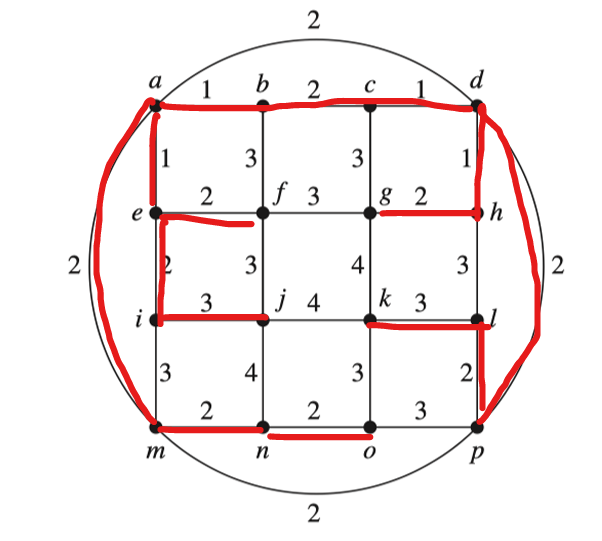
\includegraphics[width=0.4\textwidth]{屏幕截图 2024-12-22 104712.png}
    \caption{Prim's algorithm}
\end{figure}

\section{}

\begin{enumerate}
    \item Add a -- b.
    \item Add c -- d.
    \item Add d -- h.
    \item Add a -- e.
    \item Add e -- f.
    \item Add g -- h.
    \item Add a -- d.
    \item Add d -- p.
    \item Add a -- m.
    \item Add e -- i.
    \item Add m -- n.
    \item Add n -- o.
    \item Add i -- j.
    \item Add o -- k.
    \item Add k -- l.
\end{enumerate}

\begin{figure}[htbp]
    \centering
    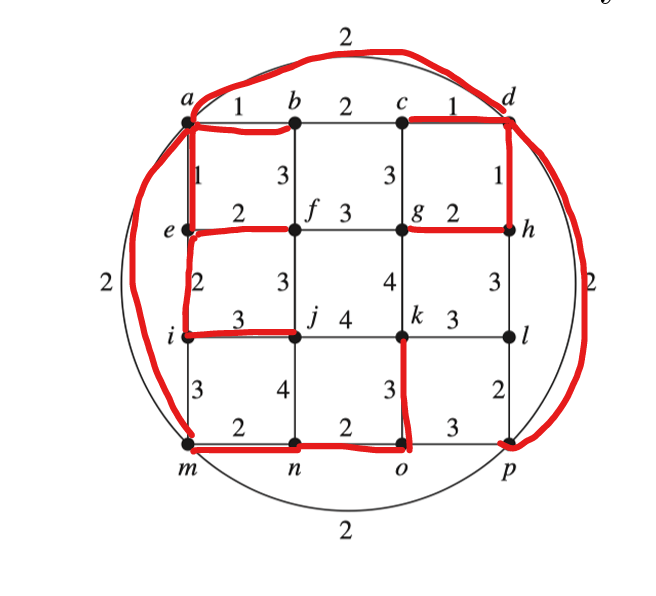
\includegraphics[width=0.4\textwidth]{屏幕截图 2024-12-22 104129.png}
    \caption{Kruskal's algorithm}
\end{figure}

\section{}

\begin{proof}
    Assuming that $T, T'$ is a minimal spanning tree of $G$, $T \neq T'$.\\
    The shortest edge in $G$ must both in $T$ and $T'$, or add the edge to form a circle and delete one of the other longer edge, the total weight will decrease, impossible. \\
    Let $G^* = T \cap T'$, obviously $T, T'$ are both the minimal spanning tree of $G^*$. Delete the commom edges of $T$ and $T'$, there will be some disconnected components. At least in one component $T$ and $T'$ are different, and the part of $T$ and $T'$ are the minimum spanning tree of the component. \\
    In such a component, repeat the step above, until the chosen part has only 2 vertexes. And due to all the edge weight are different, there must be one unique minimum spanning tree between the two vertexes, impossible! \\
    So there exists only one minimum spanning tree in the graph.
\end{proof}

\end{document}